\documentclass[aps,prl,onecolumn,superscriptaddress,nofootinbib]{revtex4-2}
\usepackage{graphicx}
\usepackage{amsmath,amssymb}
\usepackage{bm}
\usepackage[colorlinks=true,linkcolor=blue,citecolor=blue,urlcolor=blue]{hyperref}

% let figures and tables share pages with text instead of collecting on float-only pages
\setcounter{topnumber}{3}
\setcounter{bottomnumber}{2}
\setcounter{totalnumber}{4}
\renewcommand{\topfraction}{0.9}
\renewcommand{\bottomfraction}{0.8}
\renewcommand{\textfraction}{0.07}
\renewcommand{\floatpagefraction}{0.85}

\begin{document}

	\title{Crypto Statistical Arbitrage}
	\author{Yunzhe Liu}
	\affiliation{Wall Street Quants course project}
	\date{November 2026}

	\begin{abstract}
		We study momentum and reversal strategies on Binance global cryptocurrencies, net of 20~bps per unit traded, with Sharpe ratios computed on daily returns and annualized with $\sqrt{252}$. The main universe is point in time: each month, the 30 coins with the highest dollar volume over the previous 90 days, including coins that were later delisted and excluding stablecoins. Every choice is made on a training period (April 2021 -- August 2025) and the result is tested once on September 2025 -- October 2026. A risk-parity combination of cross-sectional momentum, time-series momentum, a fire-sale reversal and betting-against-beta (BAB) earns a net Sharpe ratio of 1.15 in training (beta to BTC 0.05, alpha $t$-statistic 2.7) and 0.32 in the test (2.58 in September--December 2025, $-0.72$ in 2026). Cross-sectional momentum kept working in 2026 (Sharpe 1.09), whereas it failed with the 13 coins ($-1.13$); the weak 2026 comes from BAB ($-2.8$), whose low-beta premium reversed while risk parity gave it about 41\% of the capital. The same method applied to the 13 coins gives 1.41 in training and 0.84 in the test, but the 13 coins were chosen with full-sample volume. A 30\% cap per strategy costs nothing in training and halves the 2026 damage in the 30-coin universe, but does not help with 13 coins, where the failing strategy held little capital.
	\end{abstract}%

	\maketitle

	% =====================================================================

	\section{Data, universe and backtest conventions}
	\label{sec:data}

	\textit{Data.} Hourly klines for all USDT spot pairs are downloaded from Binance's public archive (\texttt{data.binance.vision}) for January 2020 -- October 2026 and resampled to 4-hour bars. Binance global trades roughly $1000\times$ the volume of Binance.US, whose volume collapsed in 2026.

	\textit{Point-in-time universe (main results).} Leveraged tokens, fiat, wrapped tokens and stablecoins or pegged assets are excluded, using a list and a data rule: a coin whose daily closes over the past 90 days stay within a 4\% range is treated as pegged. At the start of each month, the coins are ranked on their average daily dollar volume over the previous 90 days (at least 60 days of data, traded the day before) and the top 30 form the universe for the month. 216 different coins enter the universe over time and about 4 are replaced each month. Coins that later collapsed or were delisted (LUNA, FTT, MATIC, ...) are included, so there is no survivorship bias, and a ticker re-used for a new coin (LUNA after May 2022) is split into two coins.

	\textit{13-coin universe (comparison).} A fixed set of 13 large coins (BTC, ETH, SOL, ADA, BNB, DOGE, VET, LTC, AVAX, ATOM, XLM, LINK, HBAR), chosen with full-sample Binance.US volume, on the same Binance global data. Their selection uses future information: they are coins that stayed liquid until 2025.

	\textit{Train / test split.} Warm-up April 2020 -- March 2021 (signals and risk-parity weights need history); \textbf{training April 2021 -- August 2025}, on which every choice is made with the data cut at 31 August 2025; \textbf{test September 2025 -- October 2026} (426 days), run with the same code and parameters. Several choices were made with decision rules fixed before looking at the result and executed in code (Sections~\ref{sec:ts}, \ref{sec:bab}, \ref{sec:combo}).

	\textit{Backtest.} Let $r_{i,t}$ be the return of coin $i$ over the 4-hour bar $t$, $\mathcal U_t$ the universe at bar $t$, $N_t = |\mathcal U_t|$, and $m_t = N_t^{-1}\sum_{i \in \mathcal U_{t-1}} r_{i,t}$ the return of the \emph{equal-weight market}. Let $w_{i,t}$ be the target weight decided at the close of bar $t$, with $w_{i,t} = 0$ for $i \notin \mathcal U_t$. Signals are computed for all coins, then \emph{ranked among the coins of the universe only}; unless stated otherwise, weights are demeaned ranks scaled so that $\sum_i |w_{i,t}| = 1$ (dollar neutral). The position is held from bar $t+\ell$ with $\ell \ge 1$, so there is no look-ahead, and
	\begin{equation}
		\mathrm{TO}_t = \sum_i \left| w_{i,t} - w_{i,t-1} \right|, \qquad
		r^{\mathrm{gross}}_t = \sum_i w_{i,t-\ell}\, r_{i,t}, \qquad
		r^{\mathrm{net}}_t = r^{\mathrm{gross}}_t - c\, \mathrm{TO}_{t-\ell} ,
		\label{eq:backtest}
	\end{equation}
	with $c = 20$~bps (7~bps commission and 13~bps slippage). A coin leaving the universe is sold, so the cost of replacing coins is included in turnover. A coin that stops trading is closed at its last price; from the next bar its weight is set to zero and the remaining long and short weights are rescaled separately. The \emph{break-even cost} $\overline{r^{\mathrm{gross}}} / \overline{\mathrm{TO}}$ is the largest cost per unit traded at which a strategy still breaks even.

	\textit{Statistics.} Following the course convention, 4-hour returns are summed into daily returns $d_\tau$, and
	\begin{equation}
		\mathrm{SR} = \frac{\bar d}{s_d}\sqrt{252}, \qquad
		d_\tau = \beta f_\tau + \alpha + e_\tau ,
		\label{eq:sharpe}
	\end{equation}
	where $\bar d$ and $s_d$ are the mean and standard deviation of daily net returns. Beta and alpha come from a regression of daily net returns on a daily factor $f_\tau$ (BTC or the equal-weight market).

	% =====================================================================
	\section{Momentum: horizon, costs and execution}
	\label{sec:momentum}

	\textit{Horizon.} Cross-sectional (XS) momentum ranks the coins of the universe on their average return over the last $h$ hours,
	\begin{equation}
		w_{i,t} \propto \operatorname{rank}_{i \in \mathcal U_t}\big(\bar r^{(h)}_{i,t}\big) - \overline{\operatorname{rank}}_t ,
		\label{eq:xs}
	\end{equation}
	where $\bar r^{(h)}_{i,t}$ is the average 4-hour return of coin $i$ over the last $h$ hours and $\overline{\operatorname{rank}}_t$ the mean rank. Without a skip ($\ell = 1$), short horizons are negative ($h = 4$: $-1.38$ with 30 coins, $-1.34$ with 13): over a few hours coins reverse. Skipping one bar ($\ell = 2$) makes every horizon positive [Fig.~\ref{fig:horizon}], so all momentum signals use a one-bar skip. With 30 coins the slow horizons $h = 336$ and 720 (1.20, 1.16) are positive in every training year; with 13 coins most slow horizons were already negative in January--August 2025 ($h = 168$: $-0.50$, $h = 720$: $-0.35$).

	\begin{figure}[!htbp]
		\centering
		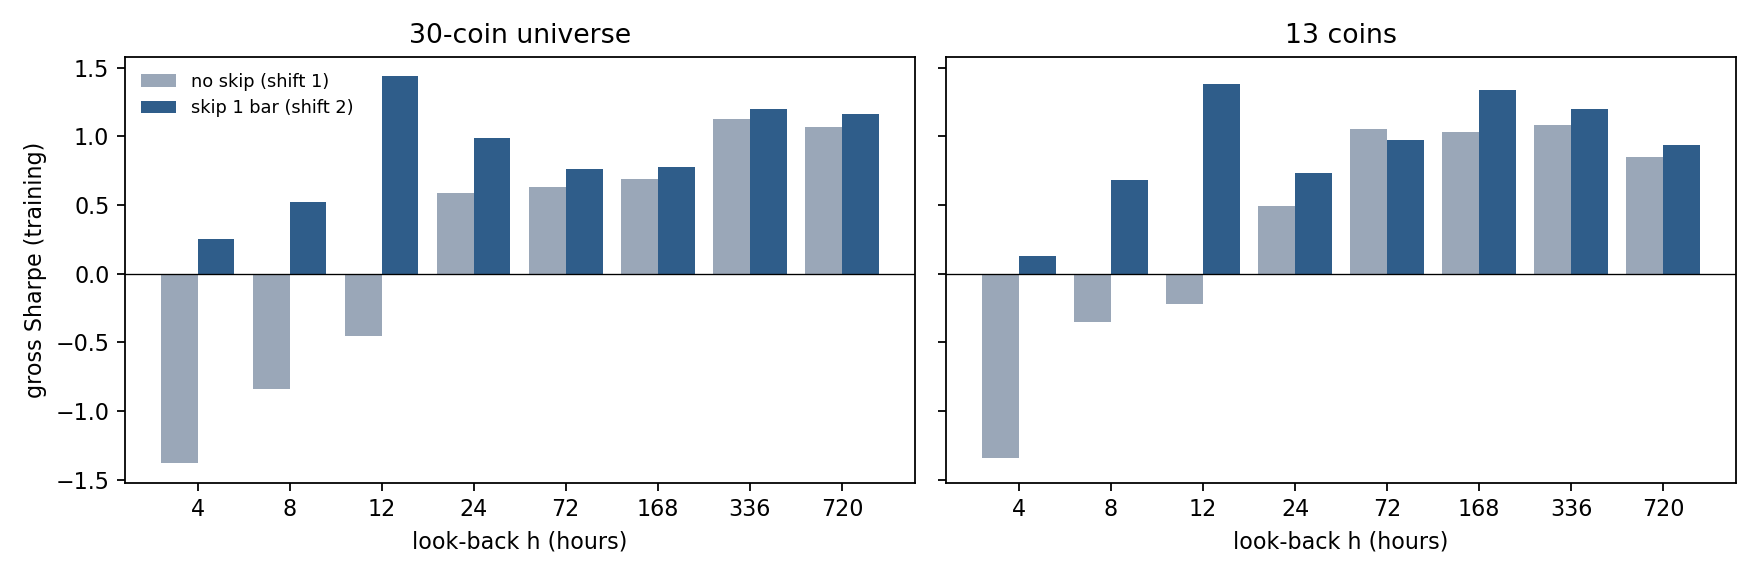
\includegraphics[width=0.95\linewidth]{figures/g1_horizon.png}
		\caption{Gross Sharpe ratio of XS momentum by look-back horizon, with and without skipping the most recent bar (training period).}
		\label{fig:horizon}
	\end{figure}

	\textit{Costs.} Rebalanced every 4 hours, every horizon loses money after costs (Table~\ref{tab:costs}): the signal works; the problem is turnover.

	\begin{table}[!htbp]
		\caption{XS momentum rebalanced every 4 hours (training period).}
		\label{tab:costs}
		\begin{ruledtabular}
			\begin{tabular}{llcccc}
				Universe & Horizon & Gross Sharpe & Net Sharpe (20 bps) & Turnover per bar & Break-even (bps) \\
				\hline
				30 coins & $h = 24$  & 0.99 & $-6.74$ & 0.550 & 2.5 \\
				& $h = 168$ & 0.78 & $-2.32$ & 0.221 & 5.0 \\
				& $h = 720$ & 1.16 & $-0.39$ & 0.109 & 14.9 \\
				13 coins & $h = 24$  & 0.73 & $-7.41$ & 0.573 & 1.7 \\
				& $h = 168$ & 1.34 & $-1.92$ & 0.232 & 8.2 \\
				& $h = 720$ & 0.94 & $-0.74$ & 0.113 & 11.2 \\
			\end{tabular}
		\end{ruledtabular}
	\end{table}

	\textit{Execution.} Rebalancing once a day (00:00~UTC) makes the slow signal positive ($h = 720$: 0.47 net with 30 coins, break-even 36~bps). We then solve, every day,
	\begin{equation}
		\min_{\bm w}\; (\bm w - \bm w^{*})^{\top} \bm\Sigma\, (\bm w - \bm w^{*}) + \lambda\, c\, \lVert \bm w - \bm w' \rVert_1
		\quad \text{s.t.} \quad \textstyle\sum_i w_i = 0,\;\; \lVert \bm w \rVert_1 \le 1,
		\label{eq:opt}
	\end{equation}
	over the coins of today's universe, where $\bm w^{*}$ is the momentum portfolio, $\bm\Sigma$ a Ledoit--Wolf covariance of the past 30 days and $\bm w'$ the position actually held (Table~\ref{tab:opt}). $\lambda = 0$ reproduces the daily rule; $\lambda = 0.003$ halves turnover and is the best value in both universes for $h = 720$. Coin replacement accounts for 4--8\% of turnover.

	\begin{table}[!htbp]
		\caption{XS momentum ($h = 720$), daily rebalance with the optimization of Eq.~(\ref{eq:opt}), training period.}
		\label{tab:opt}
		\begin{ruledtabular}
			\begin{tabular}{ccccccc}
				& \multicolumn{3}{c}{30 coins} & \multicolumn{3}{c}{13 coins} \\
				$\lambda$ & Net Sharpe & Turnover & Break-even (bps) & Net Sharpe & Turnover & Break-even (bps) \\
				\hline
				0     & 0.47 & 0.043 & 36  & 0.37 & 0.044 & 31 \\
				0.001 & 0.63 & 0.028 & 52  & 0.51 & 0.030 & 42 \\
				0.003 & \textbf{0.78} & 0.019 & 77  & \textbf{0.63} & 0.019 & 63 \\
				0.01  & 0.67 & 0.009 & 107 & 0.36 & 0.008 & 72 \\
			\end{tabular}
		\end{ruledtabular}
	\end{table}

	\textit{Improved signal.} The ideal portfolio averages the ranks of three horizons and ranks coins on volatility-adjusted returns,
	\begin{equation}
		w^{*}_{i,t} \propto \frac{1}{3} \sum_{h \in \{168,\,336,\,720\}} \operatorname{rank}_{i \in \mathcal U_t}\!\left( \frac{\bar r^{(h)}_{i,t}}{\hat\sigma_{i,t}} \right) - \overline{\operatorname{rank}}_t ,
		\label{eq:mhva}
	\end{equation}
	where $\hat\sigma_{i,t}$ is the standard deviation of the 4-hour returns of coin $i$ over the past 30 days. With the optimizer ($\lambda = 0.003$) the net Sharpe rises to \textbf{1.02} with 30 coins (break-even 66~bps) and 0.84 with 13 [Fig.~\ref{fig:costs}]. The volatility adjustment is what matters with 30 coins (daily $h = 720$: 0.47 $\to$ 0.72), because many newly listed coins are very volatile and would otherwise sit at the extremes of the ranking; with 13 coins of similar volatility it alone does not help (0.37 $\to$ 0.24). This is the final XS strategy in both universes.

	\begin{figure}[!htbp]
		\centering
		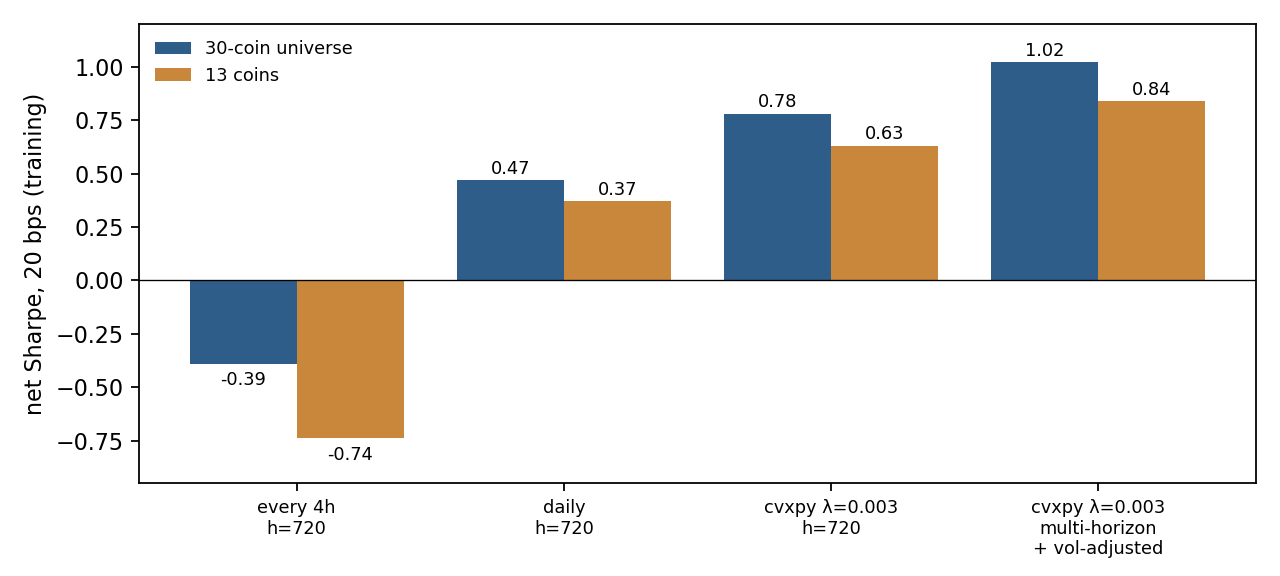
\includegraphics[width=0.75\linewidth]{figures/g2_costs.png}
		\caption{Net Sharpe ratio (20~bps) of XS momentum under successive execution improvements, training period.}
		\label{fig:costs}
	\end{figure}

	% =====================================================================
	\section{Momentum and activity (volume)}
	\label{sec:volume}

	Abnormal volume is defined relative to each coin's own history, $\mathrm{avol}_{i,t} = \overline{V}_{i,t}^{(h)} / \overline{V}_{i,t}^{(90\,\mathrm{d})}$, where $\overline{V}_{i,t}^{(x)}$ is the average 4-hour dollar volume over the last $x$. The coins of the universe are split at the median of $\mathrm{avol}$ into a high-volume half $\mathcal H_t$ and a low-volume half $\mathcal L_t$, and four signals are compared: \emph{plain} momentum [Eq.~(\ref{eq:xs})], momentum \emph{inside $\mathcal H_t$ only}, \emph{inside $\mathcal L_t$ only}, and \emph{volume-weighted} momentum, $w_{i,t} \propto (\operatorname{rank}_i(\bar r^{(h)}_{i,t}) - \overline{\operatorname{rank}}_t)(1 + p_{i,t})$ with $p_{i,t}$ the percentile of $\mathrm{avol}_{i,t}$.

	\begin{table}[!htbp]
		\caption{Volume-conditioned XS momentum, $h = 720$, training period.}
		\label{tab:volume}
		\begin{ruledtabular}
			\begin{tabular}{lcccc}
				& \multicolumn{2}{c}{30 coins} & \multicolumn{2}{c}{13 coins} \\
				Signal & Gross (every 4h) & Net, 20 bps (daily) & Gross (every 4h) & Net, 20 bps (daily) \\
				\hline
				Plain momentum   & 1.16 & 0.47 & 0.94 & 0.37 \\
				High avol only   & 1.19 & 0.57 & 0.71 & 0.01 \\
				Low avol only    & 0.94 & 0.15 & 0.20 & $-0.34$ \\
				Volume-weighted  & 1.12 & 0.44 & 0.94 & 0.35 \\
			\end{tabular}
		\end{ruledtabular}
	\end{table}

	Consistent with the hypothesis that activity strengthens momentum, momentum among high-volume coins beats low-volume coins in both universes (also for $h = 168$: 0.88 vs $-0.07$ with 30 coins). With 30 coins (15 per half) the high-volume half even beats plain momentum after costs (0.57 vs 0.47); with 13 coins (6--7 per half) splitting costs too much diversification (Table~\ref{tab:volume}). Volume is not used in the final strategy; it is the most promising extension to test on new data.

	% =====================================================================
	\section{Time-series momentum}
	\label{sec:ts}

	Time-series (TS) momentum goes long or short all coins of the universe (equal weight) according to the trend of the equal-weight market,
	\begin{equation}
		s_t = \frac14 \sum_{L \in \{7,14,30,60\}} \operatorname{sign}\!\Big(\sum_{j<6L} m_{t-j}\Big), \qquad
		w_{i,t} =
		\begin{cases}
			s_t / N_t & i \in \mathcal U_t \\
			0 & \text{otherwise,}
		\end{cases}
		\label{eq:ts}
	\end{equation}
	rebalanced daily with a one-bar skip. Table~\ref{tab:ts} compares it with three alternatives: the trend of BTC instead of the market (traded on the market or on BTC alone), and a market signal built from the \emph{current} coins' own past returns (A2), which differs from Eq.~(\ref{eq:ts}) only after a change of the universe. A2 replaces Eq.~(\ref{eq:ts}) only if its net Sharpe is at least 0.1 higher, a rule fixed in advance; it is not (Table~\ref{tab:ts}).

	\begin{table}[!htbp]
		\caption{TS momentum, average 7--60~d signal, net Sharpe (20 bps), training period.}
		\label{tab:ts}
		\begin{ruledtabular}
			\begin{tabular}{lcc}
				Signal $\to$ traded & 30 coins & 13 coins \\
				\hline
				\textbf{Market $\to$ market}, Eq.~(\ref{eq:ts}) & \textbf{0.25} & \textbf{0.53} \\
				BTC $\to$ market          & 0.15 & 0.41 \\
				BTC $\to$ BTC             & 0.03 & 0.03 \\
				Current coins (A2) $\to$ market & 0.23 & 0.53 \\
			\end{tabular}
		\end{ruledtabular}
	\end{table}

	BTC is not a better trend indicator. TS is weak with 30 coins (vol 54\%, max drawdown $-0.63$) but has a low correlation with XS (0.15) and a negative beta, because it is short in falling markets. It is much stronger with 13 coins, for a reason discussed in Section~\ref{sec:compare}.

	% =====================================================================
	\section{Reversal}
	\label{sec:reversal}

	\textit{Short-horizon reversal} (Eq.~(\ref{eq:xs}) with $h = 4$, sign flipped, no skip, every 4 hours) is real but tiny. \textit{Pairs trading} trades every pair $(A, B)$ of coins of the universe on its log-price spread, with a 30-day rolling hedge ratio $\beta_t$:
	\begin{equation}
		u_t = \log P_{A,t} - \beta_t \log P_{B,t}, \qquad
		z_t = \frac{u_t - \bar u_t}{\sigma_{u,t}}, \qquad
		q_t =
		\begin{cases}
			-1 & z_t > 2.5 \\
			+1 & z_t < -2.5 \\
			\phantom{+}0 & |z_t| < 0.5 \\
			q_{t-1} & \text{otherwise,}
		\end{cases}
		\label{eq:pairs}
	\end{equation}
	with weights $w_A = q_t/(1+|\beta_t|)$, $w_B = -q_t\beta_t/(1+|\beta_t|)$; a pair can only be open while both coins are in the universe, and the strategy averages over the eligible pairs (435 with 30 coins). Table~\ref{tab:reversal} also reports the 13 coins on Binance.US data.

	\begin{table}[!htbp]
		\caption{Reversal strategies, training period.}
		\label{tab:reversal}
		\begin{ruledtabular}
			\begin{tabular}{llccc}
				Strategy & Universe / data & Gross Sharpe & Net Sharpe (20 bps) & Break-even (bps) \\
				\hline
				4h cross-sectional reversal & 13 coins, Binance.US     & 3.34 & $-16.36$ & 3.6 \\
				& 13 coins, Binance global & 1.34 & $-19.73$ & 1.4 \\
				& 30 coins, Binance global & 1.38 & $-18.89$ & 1.4 \\
				Pairs trading & 13 coins, Binance.US     & 0.78 & 0.15    & 25 \\
				& 13 coins, Binance global & 0.59 & $-0.12$ & 17 \\
				& 30 coins, Binance global & 0.01 & $-0.76$ & 0.1 \\
				Fire sale ($k = 2$, hold 24h) & 13 coins, Binance global & 1.19 & 1.01 & 127 \\
				& 30 coins, Binance global & 0.61 & 0.44 & 71 \\
			\end{tabular}
		\end{ruledtabular}
	\end{table}

	Prices on Binance.US and Binance global are 97--100\% correlated, yet pairs trading earns exactly the small part where they differ: stale prices of thin Binance.US coins mean-revert by construction. On clean data pairs trading does not survive costs, with 13 or 30 coins.

	\textit{Fire sale (FS).} If the 24-hour equal-weight market return falls below $-k$ standard deviations of its normal 24-hour volatility, the strategy buys the whole universe (equal weight) and holds for 24 hours,
	\begin{equation}
		z_t = \frac{\sum_{j<6} m_{t-j}}{\sqrt{6}\,\hat\sigma_{m,t}}, \qquad
		w_{i,t} =
		\begin{cases}
			1 / N_t & i \in \mathcal U_t \text{ and } z_s < -k \text{ for some } s \in \{t-5, \dots, t\} \\
			0 & \text{otherwise,}
		\end{cases}
		\label{eq:fs}
	\end{equation}
	with $\hat\sigma_{m,t}$ the 90-day volatility of $m_t$. In the 24 hours after a crash the 30-coin market earns 16.9~bps per 4-hour bar versus 0.6~bps on average, so the profit is reversal, not drift. It is positive for every threshold ($k = 1.5, 2, 2.5$), holding period (12--48h) and entry delay tested; $k = 2$ is kept rather than the best cell of the grid. It lost in 2022 (crashes that kept going: LUNA, FTX) and in January--August 2025.

	% =====================================================================
	\section{Betting against beta}
	\label{sec:bab}

	Following Frazzini and Pedersen~\cite{frazzini2014}, investors who cannot or will not use leverage buy high-beta assets, which lowers their future returns. On the first day of each month, $\beta_{i,t}$ is the beta of coin $i$ to the equal-weight market over the past 90 days; among the coins of the universe, the strategy goes long the low-beta half $\mathcal B^{\mathrm{lo}}_t$ and short the high-beta half $\mathcal B^{\mathrm{hi}}_t$, each leg scaled by the inverse of its average beta,
	\begin{equation}
		w_{i,t} \propto
		\begin{cases}
			\phantom{-}1 / (n^{\mathrm{lo}}_t\, \bar\beta^{\mathrm{lo}}_t) & i \in \mathcal B^{\mathrm{lo}}_t \\
			-1 / (n^{\mathrm{hi}}_t\, \bar\beta^{\mathrm{hi}}_t) & i \in \mathcal B^{\mathrm{hi}}_t \\
			\phantom{-}0 & \text{otherwise,}
		\end{cases}
		\label{eq:bab}
	\end{equation}
	scaled to $\sum_i |w_{i,t}| = 1$ and held for one month. With 30 coins the net Sharpe is \textbf{0.63} (beta 0.04, 0.62 after removing the market, break-even 236~bps); with 13 coins it is only 0.19. Betas to BTC instead of the market give lower Sharpe ratios and fail the same 0.1 rule (Table~\ref{tab:bab}).

	\begin{table}[!htbp]
		\caption{BAB, net Sharpe (20 bps), training period.}
		\label{tab:bab}
		\begin{ruledtabular}
			\begin{tabular}{lcc}
				Beta to & 30 coins & 13 coins \\
				\hline
				\textbf{Equal-weight market}, Eq.~(\ref{eq:bab}) & \textbf{0.63} & \textbf{0.19} \\
				BTC                                           & 0.28 & $-0.16$ \\
			\end{tabular}
		\end{ruledtabular}
	\end{table}

	% =====================================================================
	\section{Combination and training performance}
	\label{sec:combo}

	The four strategies are combined with capital shares $a_{k,t}$,
	\begin{equation}
		r^{\mathrm{comb}}_t = \sum_{k} a_{k,t-1}\, r^{\mathrm{net}}_{k,t}, \qquad
		a_{k,t} = \frac{1/\hat\sigma_{k,t}}{\sum_{k'} 1/\hat\sigma_{k',t}} \quad \text{(risk parity)},
		\label{eq:combo}
	\end{equation}
	where $\hat\sigma_{k,t}$ is the volatility of strategy $k$ over the past year. Risk parity is compared with equal weights and with max-Sharpe weights $\bm a \propto \bm\Sigma^{-1}\bm\mu$, estimated on past data only (rolling, updated weekly) or on the training period itself (upper bound). TS stays in the combination unless removing it raises the risk-parity Sharpe by at least 0.1; it does not ($+0.05$ with 30 coins, $-0.05$ with 13).

	\begin{table}[!htbp]
		\caption{Combination methods, net Sharpe ratio, training period.}
		\label{tab:combo}
		\begin{ruledtabular}
			\begin{tabular}{lcc}
				Combination & 30 coins & 13 coins \\
				\hline
				4 strategies, equal                    & 0.88 & 1.24 \\
				4 strategies, rolling max Sharpe       & 0.99 & 1.10 \\
				3 strategies (no TS), risk parity      & 1.20 & 1.36 \\
				3 strategies (no BAB), risk parity     & 1.03 & 1.38 \\
				\textbf{4 strategies, risk parity}     & \textbf{1.15} & \textbf{1.41} \\
				4 strategies, max Sharpe (look-ahead)  & 1.25 & 1.47 \\
			\end{tabular}
		\end{ruledtabular}
	\end{table}

	The strategies are nearly uncorrelated (30 coins: largest correlation TS--FS $-0.24$, because TS is often short after a crash while FS is long). Risk parity is the best realistic method in both universes; rolling max-Sharpe weights suffer from noisy mean estimates. BAB, the least volatile strategy, receives the largest share (about 41\% with 30 coins).

	\begin{table}[!htbp]
		\caption{Final strategy (4 strategies, risk parity), training period April 2021 -- August 2025.}
		\label{tab:final}
		\begin{ruledtabular}
			\begin{tabular}{lcc}
				& 30 coins & 13 coins \\
				\hline
				Net Sharpe (20 bps)        & \textbf{1.15} & 1.41 \\
				Annual return (252 d)      & 14.0\% & 16.2\% \\
				Annual volatility          & 12.1\% & 11.5\% \\
				Max drawdown               & $-14.5\%$ & $-12.4\%$ \\
				Beta to BTC                & 0.05 & 0.06 \\
				Annual alpha vs BTC        & 12.9\% & 15.0\% \\
				$t$-stat (alpha vs BTC)    & 2.75 & 3.40 \\
			\end{tabular}
		\end{ruledtabular}
	\end{table}

	\begin{table}[!htbp]
		\caption{Net Sharpe ratio by year, 30 coins, training period (2025: January--August).}
		\label{tab:yearly}
		\begin{ruledtabular}
			\begin{tabular}{lccccc}
				Year & XS & TS & FS & BAB & Final \\
				\hline
				2021 & 1.75 & 0.27    & 0.93    & 0.41    & 1.60 \\
				2022 & 1.20 & 0.48    & $-0.24$ & 1.18    & 1.23 \\
				2023 & 0.33 & 0.73    & 1.05    & $-0.26$ & 0.72 \\
				2024 & 0.79 & 0.05    & 1.14    & 0.84    & 1.40 \\
				2025 & 0.89 & $-0.46$ & $-0.62$ & 0.94    & 0.53 \\
			\end{tabular}
		\end{ruledtabular}
	\end{table}

	% =====================================================================
	\section{Test period: September 2025 -- October 2026}
	\label{sec:test}

	The test uses the same code and parameters as training; recomputed on the full data, the training-period results are reproduced exactly.

	\begin{table}[!htbp]
		\caption{Net Sharpe ratio (20 bps) by period.}
		\label{tab:test}
		\begin{ruledtabular}
			\begin{tabular}{llccccc}
				Universe & Period & XS & TS & FS & BAB & \textbf{Final} \\
				\hline
				30 coins & Training (Apr-2021 -- Aug-2025) & 1.02 & 0.25 & 0.44 & 0.63 & \textbf{1.15} \\
				& \textbf{Test (Sep-2025 -- Oct-2026)} & 1.18 & 0.20 & 1.06 & $-1.88$ & \textbf{0.32} \\
				& \quad Sep--Dec 2025 & 1.40 & 0.76 & 1.90 & 0.98 & 2.58 \\
				& \quad 2026 Jan--Oct & 1.09 & $-0.11$ & 0.73 & $-2.82$ & $-0.72$ \\
				13 coins & Training (Apr-2021 -- Aug-2025) & 0.84 & 0.53 & 1.01 & 0.19 & \textbf{1.41} \\
				& \textbf{Test (Sep-2025 -- Oct-2026)} & $-0.32$ & 0.05 & 0.75 & 1.00 & \textbf{0.84} \\
				& \quad Sep--Dec 2025 & 1.28 & 0.06 & 2.42 & 1.42 & 3.07 \\
				& \quad 2026 Jan--Oct & $-1.13$ & 0.04 & 0.02 & 0.83 & $-0.10$ \\
			\end{tabular}
		\end{ruledtabular}
	\end{table}

	\begin{table}[!htbp]
		\caption{Final strategy (4 strategies, risk parity): regression of daily net returns on daily BTC returns.}
		\label{tab:testab}
		\begin{ruledtabular}
			\begin{tabular}{llcccc}
				Universe & Period & Net Sharpe & Beta to BTC & Annual alpha vs BTC & $t$-stat (alpha) \\
				\hline
				30 coins & Training (Apr-2021 -- Aug-2025)      & 1.15    & 0.05    & 12.9\%   & 2.75 \\
				& \textbf{Test (Sep-2025 -- Oct-2026)} & 0.32    & 0.04    & 3.0\%    & 0.51 \\
				& \quad Sep--Dec 2025                  & 2.58    & $-0.08$ & 18.8\%   & 1.63 \\
				& \quad 2026 Jan--Oct                  & $-0.72$ & 0.07    & $-5.0\%$ & $-0.80$ \\
				13 coins & Training (Apr-2021 -- Aug-2025)      & 1.41    & 0.06    & 15.0\%   & 3.40 \\
				& \textbf{Test (Sep-2025 -- Oct-2026)} & 0.84    & 0.02    & 5.8\%    & 1.16 \\
				& \quad Sep--Dec 2025                  & 3.07    & 0.01    & 21.2\%   & 2.15 \\
				& \quad 2026 Jan--Oct                  & $-0.10$ & 0.03    & $-0.5\%$ & $-0.09$ \\
			\end{tabular}
		\end{ruledtabular}
	\end{table}

	With 30 coins the final strategy earns 0.32 over the test (annual return 2.5\%, volatility 8\%, max drawdown $-12\%$, beta to BTC 0.04, alpha $t$-statistic 0.5), while the 30-coin market fell by about 53\% and BTC by about 24\% (sums of monthly returns). With 426 days the standard error of a Sharpe ratio is about 0.8, so the gap to training is about one standard error [Fig.~\ref{fig:cum30}].

	\begin{figure}[!htbp]
		\centering
		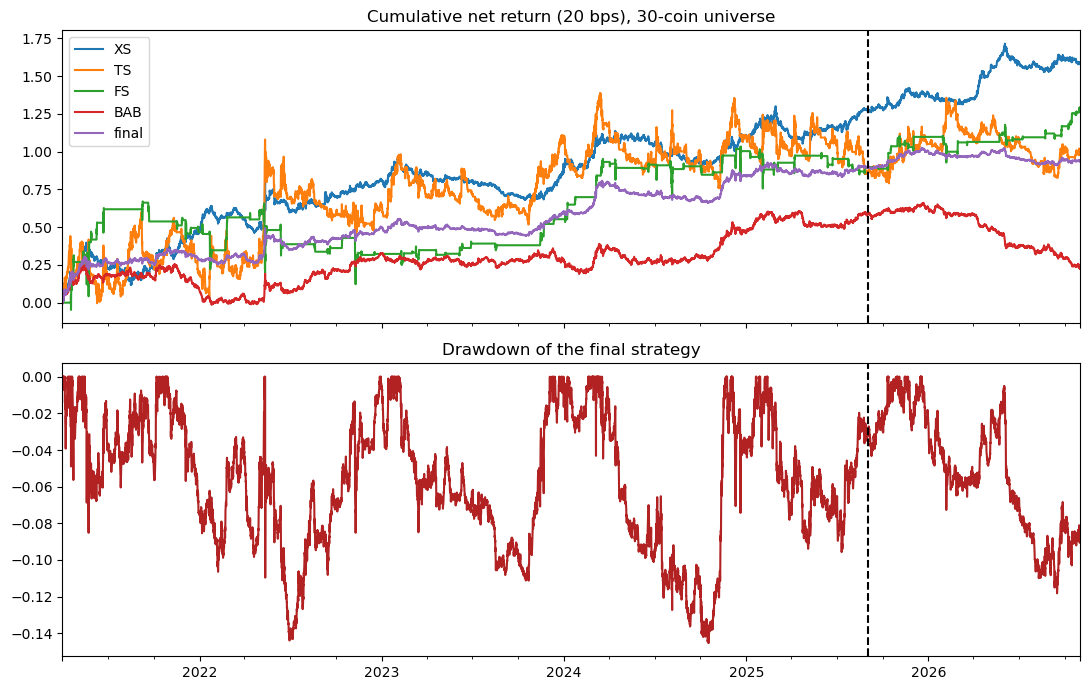
\includegraphics[width=0.85\linewidth]{figures/g3_cum30.png}
		\caption{30-coin universe: cumulative net return (summed, 20~bps) of the four strategies and the final combination, and drawdown of the combination. The dashed line marks the start of the test period.}
		\label{fig:cum30}
	\end{figure}

	\textit{Momentum did not fail with 30 coins.} XS momentum had a Sharpe of 1.09 in 2026, whereas with the 13 coins it lost ($-1.13$). Among the 13 coins, the cross-sectional dispersion of 30-day returns in 2026 was the lowest of any year (0.09), the rank correlation between past and next 30-day returns was the lowest ($-0.12$), and the market trend changed direction 23 times, the most of any year: with only large coins moving together there was no spread to earn, and a rebound inside a bear market hit the short side, the momentum crash of Daniel and Moskowitz~\cite{daniel2016}. A broader universe restored the dispersion.

	\textit{BAB failed with 30 coins.} Betas were estimated well (ex-ante 0.72 and 1.23 for the two halves in 2026, realized 0.80 and 1.20), but the beta-adjusted return (alpha against the market) of the low-beta half went from $+8.5\%$ a year in training to $-35\%$ in 2026, and the high-beta half the opposite. In rebounds the speculative high-beta coins rose far more (April 2026: $+23\%$ vs $-2\%$; September: $+41\%$ vs $+7\%$), while in sell-offs the low-beta coins fell as much (June: $-22\%$ vs $-17\%$). BAB assumes that low-beta coins move less in both directions; in 2026 they had the downside without the upside. Betas to BTC fail the same way (2026: $-3.08$, a post-hoc check). Among the 13 large coins the low-beta premium held (BAB $+0.83$). Each universe therefore exposed a different weakness, and in both the diversification across strategies limited the damage [Fig.~\ref{fig:cum13}].

	\begin{figure}[!htbp]
		\centering
		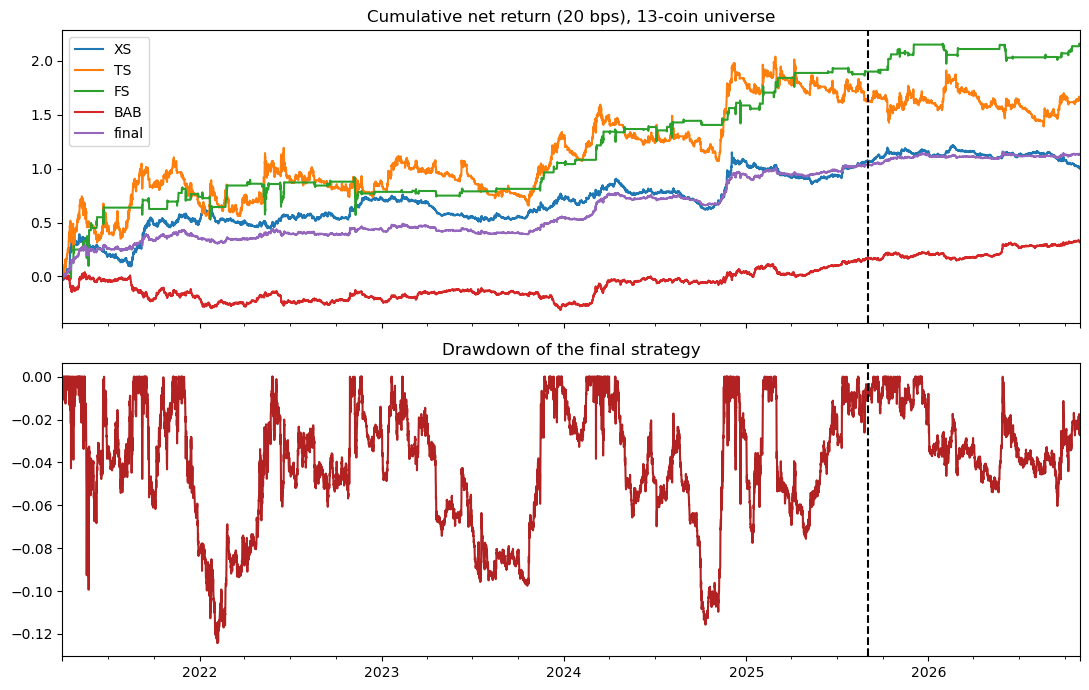
\includegraphics[width=0.85\linewidth]{figures/g4_cum13.png}
		\caption{13 coins: cumulative net return (summed, 20~bps) and drawdown of the combination. The dashed line marks the start of the test period.}
		\label{fig:cum13}
	\end{figure}

	% =====================================================================
	\section{Why the 13 coins look stronger}
	\label{sec:compare}

	With the same method, the 13-coin version has a higher training Sharpe (1.41 vs 1.15) and a higher test Sharpe (0.84 vs 0.32). The difference comes from the directional strategies: TS (0.53 vs 0.25) and fire sale (1.01 vs 0.44), while the market-neutral strategies are stronger with 30 coins (XS 1.02 vs 0.84, BAB 0.63 vs 0.19). Both TS and FS profit from the market rising: TS earns almost all of its return while long, and FS buys the market after crashes. The 13-coin market had a Sharpe of 0.53 in training against 0.11 for the 30-coin market, and rebounded more after crashes (30.9 vs 16.9~bps per 4-hour bar in the next 24 hours). This is largely survivorship: the 13 coins were chosen knowing that they stayed liquid until 2025, whereas the point-in-time universe enters coins near their volume peak and includes coins that kept falling or collapsed. The 13-coin parameters were also chosen on data overlapping the test period, and the test difference is below one standard error. The 30-coin results are therefore the main ones.

	% =====================================================================
	\section{Handling strategy failure}
	\label{sec:failure}

	Risk parity looks only at volatility, so a strategy that loses steadily at low volatility keeps its share: BAB held about 41\% of the capital throughout 2026. Two responses are compared, with shares updated daily and 20~bps paid on every change of a share: a \textbf{30\% cap} on each risk-parity share (the excess stays in cash), and \textbf{rolling max-Sharpe} weights (Section~\ref{sec:combo}), which look at past returns and therefore cut a strategy that keeps losing. They were examined after the 2026 results were known, so the test columns of Table~\ref{tab:failure} are post-hoc.

	\begin{table}[!htbp]
		\caption{Weighting methods, net Sharpe ratio. The test columns are post-hoc.}
		\label{tab:failure}
		\begin{ruledtabular}
			\begin{tabular}{llccc}
				Universe & Method & Training & Test & 2026 Jan--Oct \\
				\hline
				30 coins & Risk parity (final)  & 1.16 & 0.31 & $-0.73$ \\
				& Cap 30\%             & 1.16 & 0.62 & $-0.30$ \\
				& Rolling max Sharpe   & 0.99 & 0.90 & 0.28 \\
				& Equal weight         & 0.88 & 0.67 & $-0.12$ \\
				13 coins & Risk parity (final)  & 1.41 & 0.83 & $-0.11$ \\
				& Cap 30\%             & 1.41 & 0.75 & $-0.26$ \\
				& Rolling max Sharpe   & 1.08 & 0.66 & $-0.36$ \\
				& Equal weight         & 1.24 & 0.62 & $-0.11$ \\
			\end{tabular}
		\end{ruledtabular}
	\end{table}

	\begin{figure}[!htbp]
		\centering
		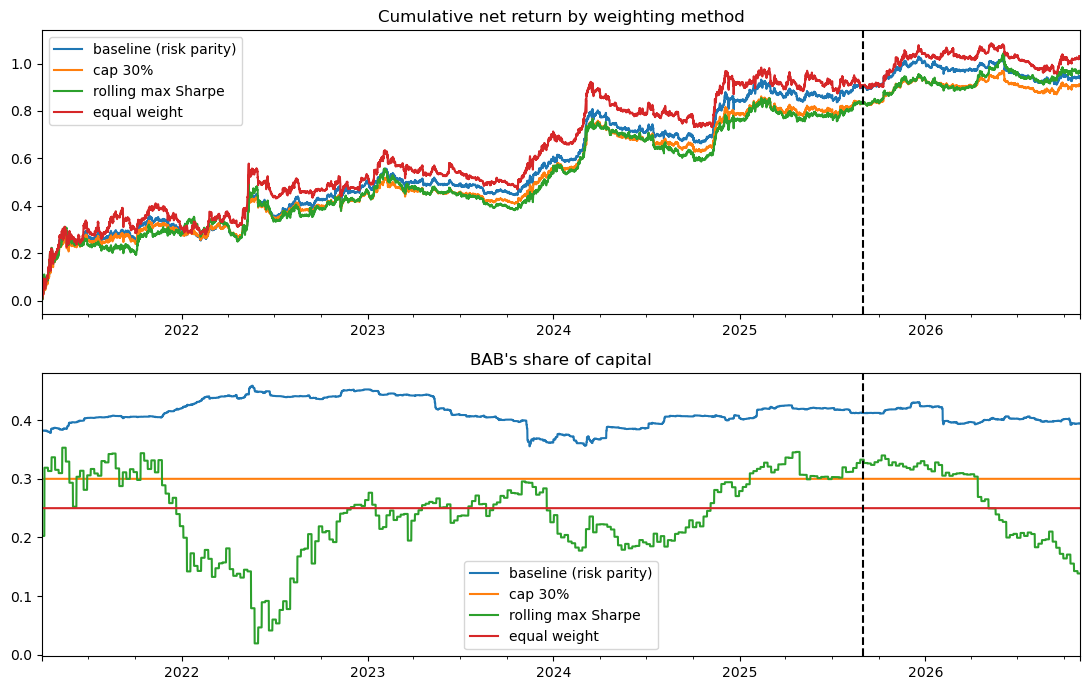
\includegraphics[width=0.85\linewidth]{figures/g5_fail30.png}
		\caption{30-coin universe: cumulative net return by weighting method, and BAB's share of capital. The dashed line marks the start of the test period.}
		\label{fig:fail30}
	\end{figure}

	\begin{figure}[!htbp]
		\centering
		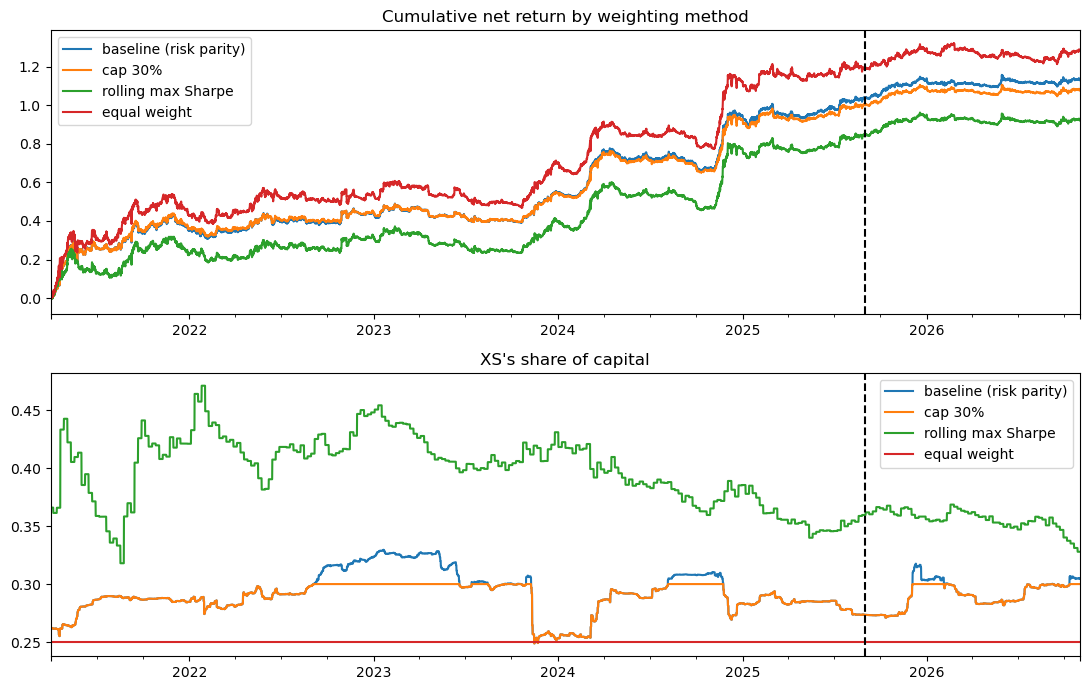
\includegraphics[width=0.85\linewidth]{figures/g6_fail13.png}
		\caption{13 coins: cumulative net return by weighting method, and XS's share of capital. The dashed line marks the start of the test period.}
		\label{fig:fail13}
	\end{figure}

	With 30 coins, the cap costs nothing in training and halves the 2026 loss; rolling max-Sharpe weights cut BAB from 33\% to 15\% during 2026 and turn the year positive, but cost 0.17 of Sharpe in training, because past mean returns are noisy [Fig.~\ref{fig:fail30}]. With 13 coins both methods make things worse: the failing strategy was XS, whose share (about 29\%) is below the cap, so the cap only trimmed BAB, which was working, and rolling max-Sharpe weights gave XS \emph{more} capital (about 36\%) because its past mean return was the highest [Fig.~\ref{fig:fail13}]. A cap and return-based weights help only when the failing strategy is the one holding the most capital; they are not a general cure. Judged on training only, the cap is the rule to adopt (no cost, and it limits concentration); it is to be evaluated on data from November 2026.

	% =====================================================================
	\section{Limitations}
	\label{sec:limits}

	The test period is short (426 days, standard error of the Sharpe ratio $\approx 0.8$) and overlaps data used to choose the 13-coin parameters; the first fully unseen data start in November 2026. Many specifications were tried on the same training data, so training Sharpe ratios are optimistic. Costs are a single 20~bps estimate; shorting requires perpetual futures or margin, whose funding costs are not modeled; weight drift between rebalances is ignored; coins that stop trading are closed at their last price, whereas the real exit price in a halt can be worse; tokenized stocks listed in 2026 are kept in the universe. The 13-coin universe uses full-sample volume (look-ahead and survivorship).

	\begin{thebibliography}{2}
		\bibitem{frazzini2014} A.~Frazzini and L.~H.~Pedersen, Betting against beta, \textit{J. Financ. Econ.} \textbf{111}, 1 (2014).
		\bibitem{daniel2016} K.~Daniel and T.~J.~Moskowitz, Momentum crashes, \textit{J. Financ. Econ.} \textbf{122}, 221 (2016).
	\end{thebibliography}

\end{document}
